\documentclass[../main.tex]{subfiles}
\begin{document}
	
	\section{Lista 4}
		\subsection{Parte 1}
		
		\begin{exercicio}{3}
			Demonstrar a propriedade operatória do limite da soma de campos vetoriais. (Baseie-se na demonstração feita no texto para o produto escalar de campos vetoriais)
		\end{exercicio}
		\begin{solucao}
			Sejam $f,g\colon S\subset \mathbb{R}^n \rightarrow \mathbb{R}^m$ campos vetoriais e $a$ ponto de acumulação de $S$. Seja $\lim_{x \to a} f(x)=b$ e $\lim_{x \to a} g(x)=c$. Pela definição de limite de funções e pela definição da soma de funções, temos:
			\begin{align*}
				\lim_{x \to a} (f(x) \pm g(x))
					&= \lim_{x \to a} (f_1(x)\pm g_1(x),\dots, f_m(x)\pm g_m(x)) \\
					&= \lim_{x \to a} \bigg((f_1(x),\dots,f_m(x))\pm (g_1(x),\dots, g_m(x))\bigg)\\
					&= \lim_{x \to a} (f_1(x),\dots,f_m(x))\pm \lim_{x \to a} (g_1(x),\dots, g_m(x)) \\
					&= \lim_{x \to a} f(x) \pm \lim_{x\to a} g(x) \\
			\end{align*}
			$\therefore \lim_{x \to a} (f(x) \pm g(x)) = b+c$
		\end{solucao}
		
		\begin{exercicio}{4}
			Exercícios da seção 8.5 do Apostol - Calc II, pp 282-283:
			\begin{enumerate}[label=\alph*)]
				\item (1) -- resolver e ilustrar em ambiente CAS;
				\item (6) -- resolver e ilustrar em ambiente CAS;
				\item (7)
				\item (8)
			\end{enumerate}
		\end{exercicio}
		\begin{solucao}
			Antes de iniciar a solução, é interessante observar as seguintes definições:
			\begin{definicao}{Limite}
				Sejam $f(x)\colon S\subset \mathbb{R}^n\to \mathbb{R}^m$, $m\geq 1$, $a\in S$ um ponto de acumulação de $S$. Dizemos que $b$ é o limite de $f(x)$ se, quando $\|x-a\|\to 0$, temos que $\|f(x)-b\|\to 0$ e escrevemos:
				\[
				\lim_{x\to a}f(x)=b
				\]
			\end{definicao}
			\begin{definicao}{Continuidade}
				Sejam $f(x)\colon S\subset \mathbb{R}^n\to \mathbb{R}^m$, $m\geq 1$, $a\in S$ um ponto de acumulação de $S$. Dizemos que $f$ é contínua em $a$ se $f$ é definida em $a$ e
				\[
				\lim_{x\to a}f(x)=f(a)
				\]
			\end{definicao}
			\begin{enumerate}[label=\alph*)]
				\item[b)] Se $(x,y)\neq (0,0)$, seja $f(x,y)=\tfrac{x^2-y^2}{x^2+y^2}$.
				Assim, note que ao longo da reta $y=mx$, temos
				\begin{align*}
					\lim_{(x,y)\to (0,0)} f(x,mx)
					&=\lim_{(x,y)\to (0,0)} \frac{x^2-m^2x^2}{x^2+m^2x^2}\\
					&=\lim_{(x,y)\to (0,0)}\frac{x^2(1-m^2)}{x^2(1+m^2)}\\
					&=\lim_{(x,y)\to (0,0)}\frac{1-m^2}{1+m^2}\\
					&=\frac{1-m^2}{1+m^2}
				\end{align*}
				Portanto, o limite de $f(x,y)$ quando $(x,y)\to (0,0)$ ao longo da reta $y=mx$ é $\tfrac{1-m^2}{1+m^2}$.
				
				No entanto, ao mesmo tempo, temos que, para a reta $x=0$, ou seja, para o eixo $y$,
				\begin{align*}
					\lim_{(x,y)\to (0,0)} f(0,y) 
					&=\lim_{(x,y)\to (0,0)} \frac{-y^2}{y^2}\\
					&=\lim_{(x,y)\to (0,0)} -1\\
					&=-1
				\end{align*}
				Analogamente, para a reta $y=0$, ou seja, para o eixo $x$,
				\begin{align*}
					\lim_{(x,y)\to (0,0)} f(x,0)
					&=\lim_{(x,y)\to (0,0)} \frac{x^2}{x^2}\\
					&=\lim_{(x,y)\to (0,0)}1\\
					&=1
				\end{align*}
				Dessa forma, note que o limite de $f(x,y)$ quando $(x,y)\to (0,0)$ é diferente, dependendo do caminho que tomamos. Logo, não existe um $b$ tal que, quando $\|(x,y)-(0,0)\|\to 0$, temos que $\|f(x,y)-b\|\to 0$, pois caso $b=1$, sempre existe uma sequência em $(x,y)$ tal que $f(x,y)$ converge para um número diferente $b_1=-1$, e vice-versa. Pela definição de limite, $\lim_{(x,y)\to (0,0)} f(x,y)$ não existe.
				
				Entretanto, note que, pela definição de continuidade num ponto $a=(0,0)$, $\lim_{(x,y)\to a} f(x,y)$ deve existir, e deve ser igual a $f(a)$. Como esse limite não existe, não é possível definir $f(0,0)$, de modo que $f$ seja contínua em $(0,0)$.
				Abaixo está a ilustração da função $f$ no SageMath.
				\begin{center}
					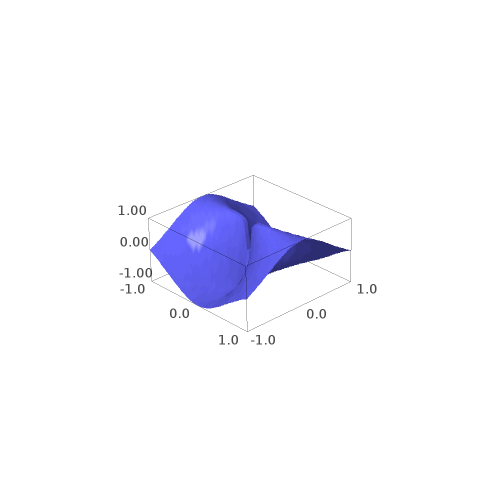
\includegraphics[width=0.25\textwidth]{imagens/lista04/picture_lista04.01_q04_item02.png}
					\captionof{figure}{$f(x,y)=\tfrac{x^2-y^2}{x^2+y^2}$}
				\end{center}
				Embora as retas $y=x$,$y=0$ e $x=0$ no plano $z=0$ não ilustrem bem o que ocorre, note que há um "abismo" na superfície, quando nos aproximamos de $0$. Além disso, dando um "zoom" no gráfico, há descontinuidades, dificilmente representadas devido à densidade dos pontos.
				\item[d)] Seja $f(x,y)=\tfrac{\sin(x^2+y^2)}{x^2+y^2}$ quando $(x,y)\neq (0,0)$. Queremos definir $f(0,0)$ de modo que $f$ seja contínua em $(0,0)$. Para tal, devemos verificar a existência do limite $\lim_{(x,y)\to (0,0)} f(x,y)$.
				
				Assim, seja $g(x,y)\coloneq x^2+y^2$ e $h(x)\coloneq \tfrac{\sin(x)}{x}$. Note que, pela continuidade dos polinômios e pelo limite trigonométrico fundamental,
				\begin{itemize}
					\item $\lim_{(x,y)\to (0,0)} g(x,y)=g(0,0)=0+0=0$
					\item $\lim_{x\to 0} h(x)=\lim_{z\to 0} \frac{\sin(x)}{x}=1$
				\end{itemize}
				Com isso, pela propriedade do limite de funções compostas,
				\begin{align*}
					\lim_{(x,y)\to (0,0)} f(x,y)
						&=\lim_{(x,y)\to (0,0)} \tfrac{\sin(x^2+y^2)}{x^2+y^2}\\
						&=\lim_{(x,y)\to (0,0)}h(g(x))=1
				\end{align*}
				Pela definição de continuidade, devemos definir $f(0,0)$ de modo que $\lim_{(x,y)\to (0,0)}f(x,y)=f(0,0)$. Assim, $f(0,0)\coloneq 1$.
			\end{enumerate}
		\end{solucao}
		\subsection{Parte 2}
		
		\begin{exercicio}{1}
			Seção 8.9, Apostol -- Cálculo 2. Exercícios 4 a 13. Resolver alguns manualmente e alguns computacionalmente.
		\end{exercicio}
		
		\begin{solucao}
			\begin{enumerate}[label=\arabic*.]
				\item[4.] Queremos calcular todas as derivadas parciais de $f$, onde $f(x,y)=x^2+y^2\sin(xy)$.
				
				\begin{align*}
					\frac{\partial f}{\partial x}(x,y)
					&=\frac{\partial x^2}{\partial x}+\frac{\partial y^2\sin(xy)}{\partial x}\\
					&=2x+y^2\frac{\partial \sin(xy)}{\partial x}\\
					&=2x+y^2\cdot y\cos(xy)=2x+y^3\cos(xy)
				\end{align*}
				\begin{align*}
					\frac{\partial f}{\partial y}(x,y)
					&=\frac{\partial x^2}{\partial y}+\frac{\partial y^2\sin(xy)}{\partial y}\\
					&=0+y^2\frac{\partial \sin(xy)}{\partial y}+\frac{\partial y^2}{\partial y}\sin(xy)\\
					&=y^2 x\cos(xy)+2y\sin(xy)\\
				\end{align*}
				Para representar computacionalmente, podemos indicar um ponto $(1,1)$, por exemplo, e plotar a superfície da função $f$, os planos que passam por esse ponto e as retas tangentes à curva gerada pela interseção dos planos com a superfície. Essas retas terão justamente inclinação igual às derivadas parciais, aplicadas no ponto escolhido.
				\begin{center}
					% Primeira imagem
					\begin{minipage}{0.45\textwidth}
						\centering
						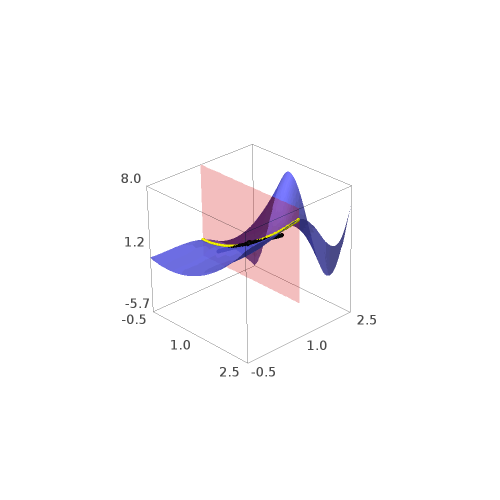
\includegraphics[width=\textwidth]{imagens/lista04/picture_lista04.02_q01_item04.01.png}
						\captionof{figure}{Questão 4, representação da derivada parcial com relação a $x$}
					\end{minipage}
					\hfill
					% Segunda imagem
					\begin{minipage}{0.45\textwidth}
						\centering
						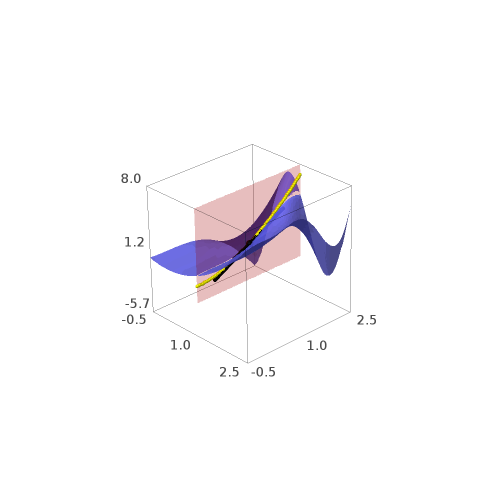
\includegraphics[width=\textwidth]{imagens/lista04/picture_lista04.02_q01_item04.02.png}
						\captionof{figure}{Questão 4, representação da derivada parcial com relação a $y$}
					\end{minipage}
				\end{center}
				\item[5.]
				Seja $f(x,y)=\sqrt{x^2 + y^2}$.
				
				Para representar computacionalmente, podemos indicar um ponto $(1,1)$, por exemplo, e plotar a superfície da função $f$, os planos que passam por esse ponto e as retas tangentes à curva gerada pela interseção dos planos com a superfície. Essas retas terão justamente inclinação igual às derivadas parciais, aplicadas no ponto escolhido.
				\begin{center}
					% Primeira imagem
					\begin{minipage}{0.45\textwidth}
						\centering
						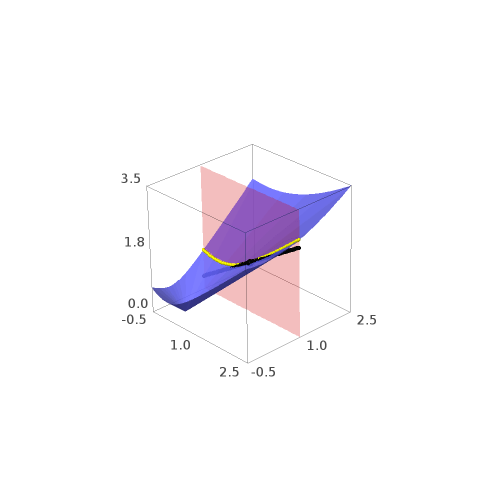
\includegraphics[width=\textwidth]{imagens/lista04/picture_lista04.02_q01_item05.01.png}
						\captionof{figure}{Questão 5, representação da derivada parcial com relação a $x$}
					\end{minipage}
					\hfill
					% Segunda imagem
					\begin{minipage}{0.45\textwidth}
						\centering
						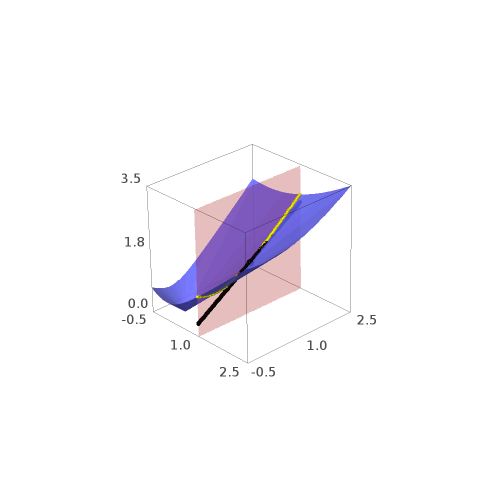
\includegraphics[width=\textwidth]{imagens/lista04/picture_lista04.02_q01_item05.02.png}
						\captionof{figure}{Questão 5, representação da derivada parcial com relação a $y$}
					\end{minipage}
				\end{center}
				\item[10.] Queremos calcular todas as derivadas parciais de $f$, onde $f(x,y)=x^4+y^4-4x^2y^2$. Além disso, queremos verificar que as derivadas parciais de segunda ordem são iguais, ou seja, que $\tfrac{\partial^2 f}{\partial x \partial y}=\tfrac{\partial^2 f}{\partial y \partial x}$.
				
				Calculando as derivadas parciais de primeira ordem:
				\begin{align*}
					\frac{\partial f}{\partial x}(x,y)
					&=\frac{\partial x^4}{\partial x}+\frac{\partial y^4}{\partial x}-4\frac{\partial x^2y^2}{\partial x}\\
					&=4x^3+0-8y^2x=4x^3-8y^2x
				\end{align*}
				\begin{align*}
					\frac{\partial f}{\partial y}(x,y)
					&=\frac{\partial x^4}{\partial y}+\frac{\partial y^4}{\partial y}-4\frac{\partial x^2y^2}{\partial y}\\
					&=0+4y^3-8x^2y=4y^3-8x^2y
				\end{align*}
				
				Calculando as derivadas parciais de segunda ordem:
				\begin{align*}
					\frac{\partial^2 f}{\partial x \partial y}(x,y)
					&=\frac{\partial 4x^3}{\partial y}-\frac{\partial 8y^2x}{\partial y}\\
					&=0-8x\cdot 2y=-16xy
				\end{align*}
				\begin{align*}
					\frac{\partial^2 f}{\partial y \partial x}(x,y)
					&=\frac{\partial 4y^3}{\partial x}-\frac{\partial -8x^2y}{\partial x}\\
					&=0-8y\cdot 2x=-16xy
				\end{align*}
				
				$\therefore \frac{\partial^2 f}{\partial xy}=\frac{\partial^2 f}{\partial yx}$ 
				
				Para representar computacionalmente, é interessante entender a derivada parcial mista como a "taxa de variação" da reta tangente mencionada nas questões anteriores (4 e 5, por exemplo). Assim, escolhendo uma variação pequena, podemos tentar visualizar uma variação semelhante tanto para a derivada parcial com relação a $\partial x \partial y$, quando a $\partial y \partial x$.
				
				\begin{center}
					% Primeira imagem
					\begin{minipage}{0.45\textwidth}
						\centering
						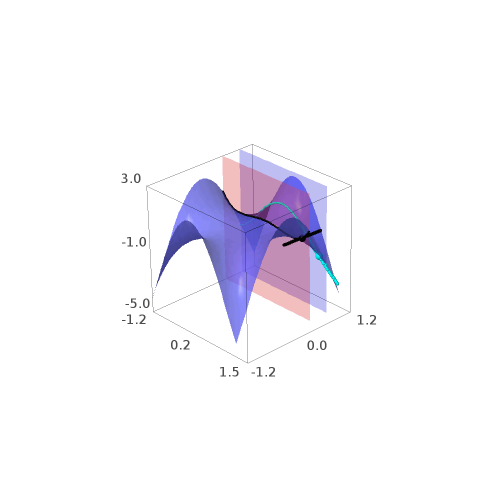
\includegraphics[width=\textwidth]{imagens/lista04/picture_lista04.02_q01_item10.01.png}
						\captionof{figure}{Questão 10, representação da derivada parcial com relação a $\partial x \partial y$}
					\end{minipage}
					\hfill
					% Segunda imagem
					\begin{minipage}{0.45\textwidth}
						\centering
						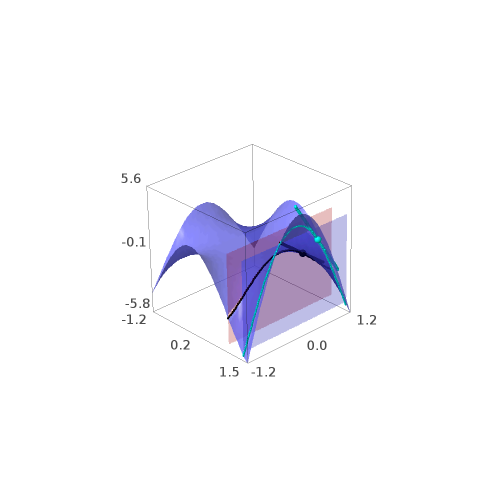
\includegraphics[width=\textwidth]{imagens/lista04/picture_lista04.02_q01_item10.02.png}
						\captionof{figure}{Questão 10, representação da derivada parcial com relação a $\partial y \partial x$}
					\end{minipage}
				\end{center}
				\item[11.]
				Seja $f(x,y)=\log(x^2+y^2)$
				
				Para representar computacionalmente, é interessante entender a derivada parcial mista como a "taxa de variação" da reta tangente mencionada nas questões anteriores (4 e 5, por exemplo). Assim, escolhendo uma variação pequena, podemos tentar visualizar uma variação semelhante tanto para a derivada parcial com relação a $\partial x \partial y$, quando a $\partial y \partial x$.
				
				\begin{center}
					% Primeira imagem
					\begin{minipage}{0.45\textwidth}
						\centering
						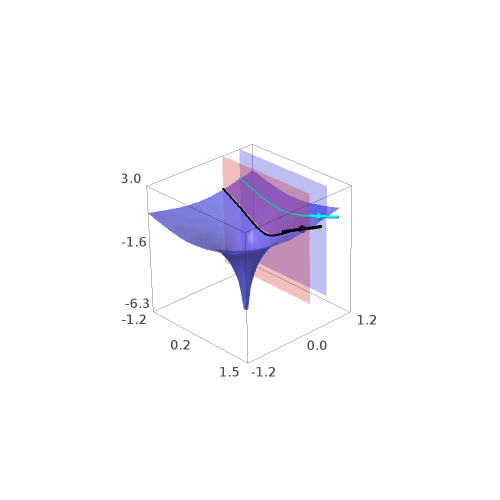
\includegraphics[width=\textwidth]{imagens/lista04/picture_lista04.02_q01_item11.01.png}
						\captionof{figure}{Questão 11, representação da derivada parcial com relação a $\partial x \partial y$}
					\end{minipage}
					\hfill
					% Segunda imagem
					\begin{minipage}{0.45\textwidth}
						\centering
						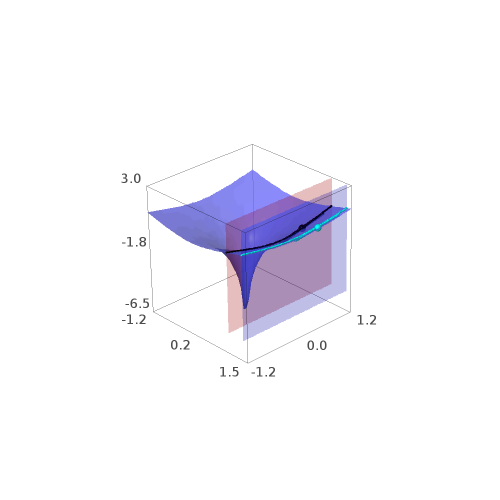
\includegraphics[width=\textwidth]{imagens/lista04/picture_lista04.02_q01_item11.02.png}
						\captionof{figure}{Questão 11, representação da derivada parcial com relação a $\partial y \partial x$}
					\end{minipage}
				\end{center}
				\item[12.]
				Seja $f(x,y)=\frac{1}{y}\cos(x^2)$
				
				Para representar computacionalmente, é interessante entender a derivada parcial mista como a "taxa de variação" da reta tangente mencionada nas questões anteriores (4 e 5, por exemplo). Assim, escolhendo uma variação pequena, podemos tentar visualizar uma variação semelhante tanto para a derivada parcial com relação a $\partial x \partial y$, quando a $\partial y \partial x$.
				
				\begin{center}
					% Primeira imagem
					\begin{minipage}{0.45\textwidth}
						\centering
						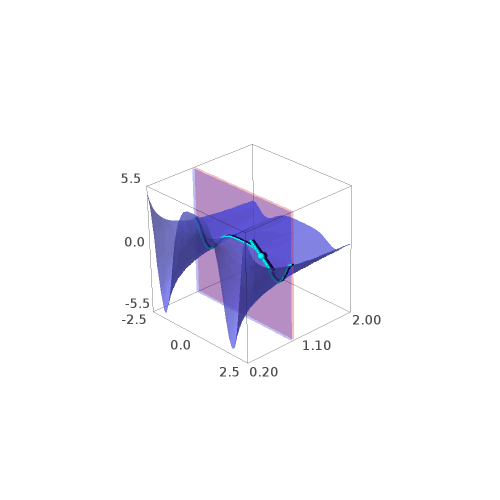
\includegraphics[width=\textwidth]{imagens/lista04/picture_lista04.02_q01_item12.01.png}
						\captionof{figure}{Questão 12, representação da derivada parcial com relação a $\partial x \partial y$}
					\end{minipage}
					\hfill
					% Segunda imagem
					\begin{minipage}{0.45\textwidth}
						\centering
						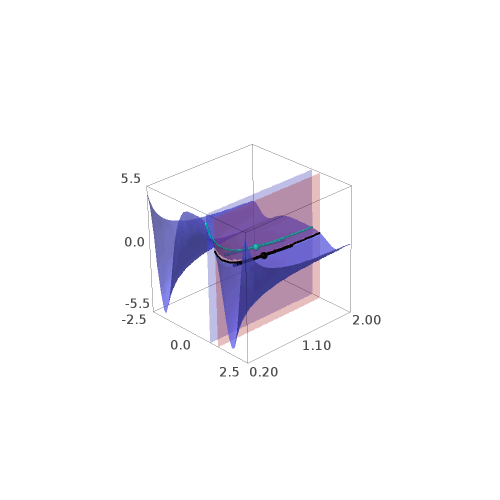
\includegraphics[width=\textwidth]{imagens/lista04/picture_lista04.02_q01_item12.02.png}
						\captionof{figure}{Questão 12, representação da derivada parcial com relação a $\partial y \partial x$}
					\end{minipage}
				\end{center}
			\end{enumerate}
		\end{solucao}
		
		\begin{exercicio}{2}
			Seção 8.14, Apostol -- Cálculo 2. Exercícios 1, 2, 3 e 7.
		\end{exercicio}
		\begin{solucao}
			\begin{enumerate}[label=\arabic.]
				\item[1.] Queremos encontrar o vetor gradiente de todos os pontos em que ele existe.
					\begin{enumerate}[label=\alph*)]
						\item Seja $f(x,y)=x^2+y^2\sin(xy)$.
							\begin{itemize}
								\item $\frac{\partial f}{\partial x}(x,y)=\frac{\partial }{\partial x}\big(x^2+y^2\sin(xy)\big)=2x+y^3\cos(xy)$
								\item $\frac{\partial f}{\partial y}(x,y)=\frac{\partial }{\partial y}\big(x^2+y^2\sin(xy)\big)=2y\sin(xy)+y^2x\cos(xy)$
							\end{itemize}
							Note que essas derivadas parciais existem em todos os pontos e, portanto, o vetor gradiente também existe em todos os pontos.
							
							$\therefore \nabla f(x,y)=\big(2x+y^3\cos(xy), 2y\sin(xy)+y^2x\cos(xy)\big)$
							
							Para a representação computacional, no campo escalar em $\mathbb{R}^2$, é possível plotar as superfícies no $\mathbb{R}^3$ e os vetores gradientes em pontos escolhidos.
							
							\begin{center}
								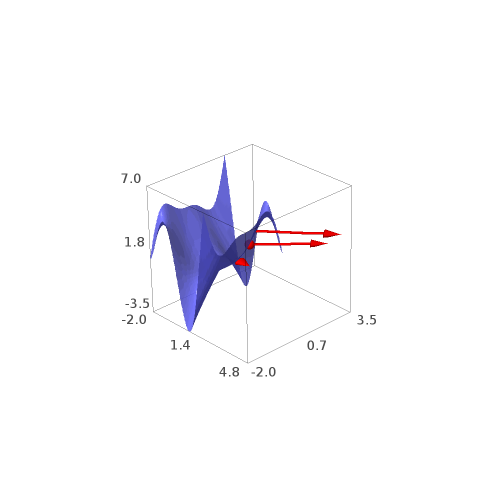
\includegraphics[width=0.25\textwidth]{imagens/lista04/picture_lista04.02_q02_item01.01.png}
								\captionof{figure}{Vetores gradientes de $f(x,y)=x^2+y^2\sin(xy)$}
							\end{center}
							
						\item Seja $f(x,y)=e^x\cos(y)$.
							\begin{itemize}
								\item $\frac{\partial f}{\partial x}(x,y)=\frac{\partial }{\partial x}\big(e^x\cos(y)\big)=\cos(y)\frac{\partial }{\partial x}\big(e^x\big)=e^x\cos(y)$
								\item $\frac{\partial f}{\partial y}(x,y)=\frac{\partial }{\partial y}\big(e^x\cos(y)\big)=e^x\frac{\partial }{\partial y}\big(\cos(y)\big)=-e^x\sin(y)$
							\end{itemize}
							Note que essas derivadas parciais existem em todos os pontos e, portanto, o vetor gradiente também existe em todos os pontos.
							
							$\therefore \nabla f(x,y)=\big(e^x\cos(y), -e^x\sin(y)\big)$
							
							Para a representação computacional, no campo escalar em $\mathbb{R}^2$, é possível plotar as superfícies no $\mathbb{R}^3$ e os vetores gradientes em pontos escolhidos.
							
							\begin{center}
								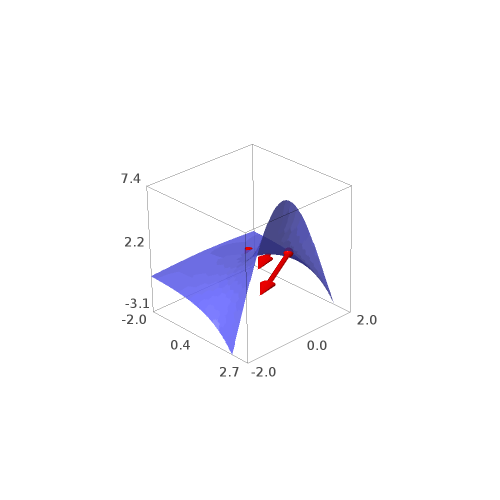
\includegraphics[width=0.25\textwidth]{imagens/lista04/picture_lista04.02_q02_item01.02.png}
								\captionof{figure}{Vetores gradientes de $f(x,y)=e^x\cos(y)$}
							\end{center}
							
						\item Seja $f(x,y,z)=x^2y^3z^4$.
						\begin{itemize}
							\item $\frac{\partial f}{\partial x}(x,y,z)=\frac{\partial }{\partial x}\big(x^2y^3z^4\big)=y^3z^4\frac{\partial }{\partial x}\big(x^2\big)=2xy^3z^4$
							\item $\frac{\partial f}{\partial y}(x,y,z)=\frac{\partial }{\partial y}\big(x^2y^3z^4\big)=x^2z^4\frac{\partial }{\partial y}\big(y^3\big)=3x^2y^2z^4$
							\item $\frac{\partial f}{\partial z}(x,y,z)=\frac{\partial }{\partial z}\big(x^2y^3z^4\big)=x^2y^3\frac{\partial }{\partial z}\big(z^4\big)=4x^2y^3z^3$
						\end{itemize}
						Note que essas derivadas parciais existem em todos os pontos e, portanto, o vetor gradiente também existe em todos os pontos.
						
						$\therefore \nabla f(x,y,z)=\big(2xy^3z^4, 3x^2y^2z^4, 4x^2y^3z^3\big)$
						
						Para a representação computacional, não é possível plotar a função $f$, devido ao seu caráter de quatro dimensões. No entanto, é possível plotar os vetores, de três dimensões, e as cuvas de nível correspondentes. Note que os vetores gradiente são "ortogonais" às curvas de nível.
						
						\begin{center}
							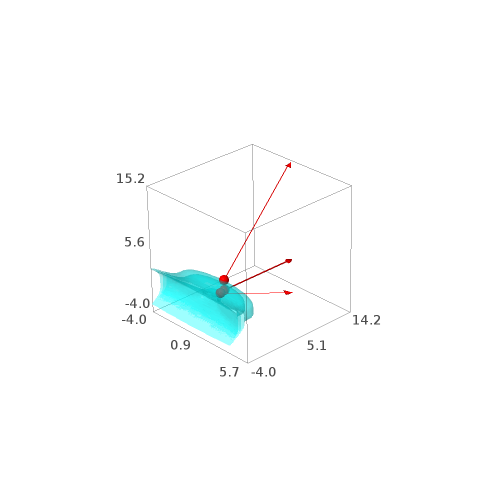
\includegraphics[width=0.25\textwidth]{imagens/lista04/picture_lista04.02_q02_item01.03.png}
							\captionof{figure}{Vetores gradientes de $f(x,y,z)=x^2y^3z^4$}
						\end{center}
						
						\item Seja $f(x,y,z)=x^2-y^2+2z^2$.
						\begin{itemize}
							\item $\frac{\partial f}{\partial x}(x,y,z)=\frac{\partial }{\partial x}\big(x^2-y^2+2z^2\big)=\frac{\partial }{\partial x}\big(x^2\big)+0+0=2x$
							\item $\frac{\partial f}{\partial y}(x,y,z)=\frac{\partial }{\partial y}\big(x^2-y^2+2z^2\big)=0-\frac{\partial }{\partial y}\big(y^2\big)+0=-2y$
							\item $\frac{\partial f}{\partial z}(x,y,z)=\frac{\partial }{\partial z}\big(x^2-y^2+2z^2\big)=0+0+2\frac{\partial }{\partial z}\big(z^2\big)=4z$
						\end{itemize}
						Note que essas derivadas parciais existem em todos os pontos e, portanto, o vetor gradiente também existe em todos os pontos.
						
						$\therefore \nabla f(x,y,z)=\big(2x,-2y,4z\big)$
						
						Para a representação computacional, não é possível plotar a função $f$, devido ao seu caráter de quatro dimensões. No entanto, é possível plotar os vetores, de três dimensões, e as cuvas de nível correspondentes. Note que os vetores gradiente são "ortogonais" às curvas de nível.
						
						\begin{center}
							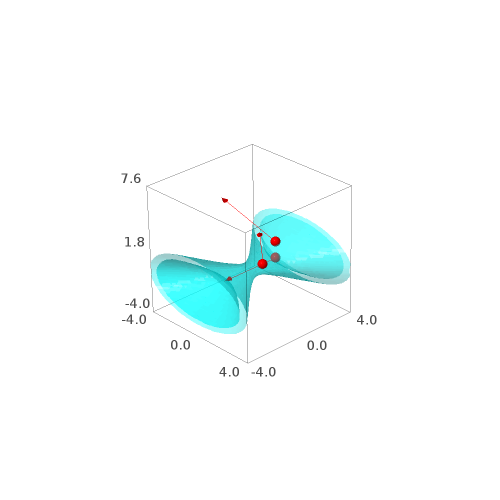
\includegraphics[width=0.25\textwidth]{imagens/lista04/picture_lista04.02_q02_item01.04.png}
							\captionof{figure}{Vetores gradientes de $f(x,y,z)=x^2-y^2+2z^2$}
						\end{center}
						
						\item Seja $f(x,y,z)=\log(x^2+2y^2-3z^2)$.
						\begin{itemize}
							\item $\frac{\partial f}{\partial x}(x,y,z)=\frac{\partial }{\partial x}\big(\log(x^2+2y^2-3z^2)\big)=\frac{\big( x^2+2y^2-3z^2\big) '}{x^2+2y^2-3z^2}=\frac{2x}{x^2+2y^2-3z^2}$
							\item $\frac{\partial f}{\partial y}(x,y,z)=\frac{\partial }{\partial y}\big(\log(x^2+2y^2-3z^2)\big)=\frac{\big(x^2+2y^2-3z^2\big) '}{x^2+2y^2-3z^2}=\frac{4y}{x^2+2y^2-3z^2}$
							\item $\frac{\partial f}{\partial z}(x,y,z)=\frac{\partial }{\partial z}\big(\log(x^2+2y^2-3z^2)\big)=\frac{\big(x^2+2y^2-3z^2\big) '}{x^2+2y^2-3z^2}=-\frac{6z}{x^2+2y^2-3z^2}$
						\end{itemize}
						Note que essas derivadas parciais existem em todos os pontos onde $x^2+2y^2-3z^2> 0$ e, portanto, o vetor gradiente é definido apenas nesses pontos.
						
						$\therefore \nabla f(x,y,z)=\big(\frac{2x}{x^2+2y^2-3z^2},\frac{4y}{x^2+2y^2-3z^2},-\frac{6z}{x^2+2y^2-3z^2}\big)$
						
						Para a representação computacional, não é possível plotar a função $f$, devido ao seu caráter de quatro dimensões. No entanto, é possível plotar os vetores, de três dimensões, e as cuvas de nível correspondentes. Note que os vetores gradiente são "ortogonais" às curvas de nível.
						
						\begin{center}
							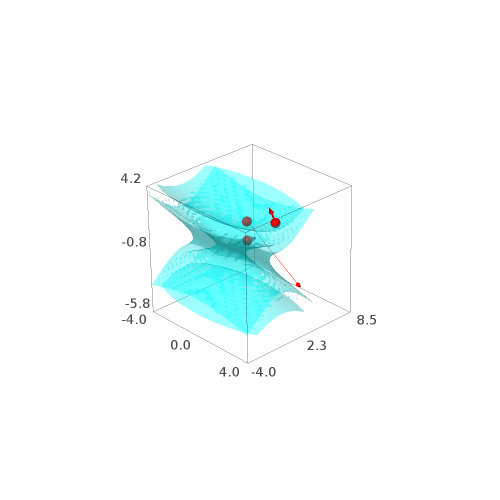
\includegraphics[width=0.25\textwidth]{imagens/lista04/picture_lista04.02_q02_item01.05.png}
							\captionof{figure}{Vetores gradientes de $f(x,y,z)=\log(x^2+2y^2-3z^2)$}
						\end{center}
						
						\item Seja $f(x,y,z)=x^{y^z}$.
						\begin{itemize}
							\item $\frac{\partial f}{\partial x}(x,y,z)=\frac{\partial }{\partial x}\big(x^{y^z}\big)=y^z\cdot x^{y^z-1}$
							\item $\frac{\partial f}{\partial y}(x,y,z)=\frac{\partial }{\partial y}\big(x^{y^z}\big)=\frac{\partial }{\partial y}\big(e^{y^z\log(x)}\big)=e^{y^z\log(x)}\cdot \frac{\partial }{\partial y}\big(y^z\log(x)\big)\\=x^{y^z}\cdot \log(x)\cdot zy^{z-1}$
							\item $\frac{\partial f}{\partial y}(x,y,z)=\frac{\partial }{\partial y}\big(x^{y^z}\big)=\frac{\partial }{\partial y}\big(e^{y^z\log(x)}\big)=e^{y^z\log(x)}\cdot \frac{\partial }{\partial y}\big(y^z\log(x)\big)\\=x^{y^z}\cdot \log(x)\cdot \frac{\partial }{\partial y}\big(e^{z\log(y)}\big)=x^{y^z}\cdot \log(x)\cdot e^{z\log(y)}\cdot \frac{\partial }{\partial y}\big(z\log(y)\big)\\=x^{y^z}\cdot \log(x)\cdot y^z\cdot \log(y)$
						\end{itemize}
						Note que essas derivadas parciais existem em todos os pontos e, portanto, o vetor gradiente também existe em todos os pontos.
						
						$\therefore \nabla f(x,y,z)=\big(y^z\cdot x^{y^z-1},x^{y^z}\cdot \log(x)\cdot zy^{z-1},x^{y^z}\cdot \log(x)\cdot y^z\cdot \log(y)\big)$
						
						Para a representação computacional, não é possível plotar a função $f$, devido ao seu caráter de quatro dimensões. No entanto, é possível plotar os vetores, de três dimensões, e as cuvas de nível correspondentes. Note que os vetores gradiente são "ortogonais" às curvas de nível.
						
						\begin{center}
							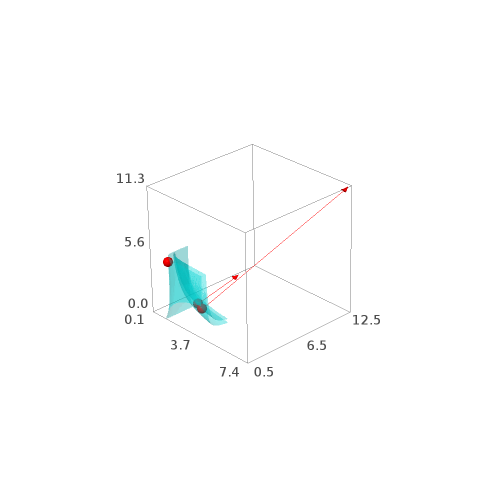
\includegraphics[width=0.25\textwidth]{imagens/lista04/picture_lista04.02_q02_item01.06.png}
							\captionof{figure}{Vetores gradientes de $f(x,y,z)=x^{y^z}$}
						\end{center}
						
					\end{enumerate}
			\end{enumerate}
		\end{solucao}
		
		\begin{exercicio}{3}
			Ilustre computacionalmente o Teorema do Valor Médio que
			tem o seguinte enunciado:
			\begin{teorema}{Teorema do Valor Médio}
				Seja $f\colon \mathbb{R}^n\to \mathbb{R}$ um campo escalar diferenciável, e $P$ e $Q$ dois pontos de $\mathbb{R}^n$. Então existe um ponto $M$ sobre o segmento de reta que liga os pontos $P$ e $Q$ tal que:
				\[
				f(Q)-f(P)=\langle \nabla f(M), Q-P\rangle
				\]
			\end{teorema}
			\textit{Dica:} Escolha um campo escalar de sua preferência e varie os pontos $P$ e $Q$ de forma a ser possível comparar $f(M)$ e $Q-P$
			
			\textbf{Observação:} o Teorema do Valor Médio não vale para funções $f\colon \mathbb{R}^n\to \mathbb{R^m}$ com $m>1$. Em particular, não vale para curvas.
		\end{exercicio} 
		\begin{solucao}
			Para ilustrar computacionalmente, podemos fazer uma animação dos pontos $P$ e $Q$ variando, como consta no arquivo .ipynb enviado em anexo junto desta lista.
			
			Outra forma de visualizar seria tomando uma função de exemplo. Assim, seja $f$ uma função tal que $f(x,y)=x^2 + xy + 2y^2$. Além disso, sejam $P=(-1,-0.3)$ e $Q=(1.2, 0.8)$. Note que a inclinação do segmento de reta $P-Q$ e da reta tangente ao ponto $M$ encontrado pelo código (também no arquivo .ipynb enviado em anexo, junto desta lista) são as mesmas.
			\begin{center}
				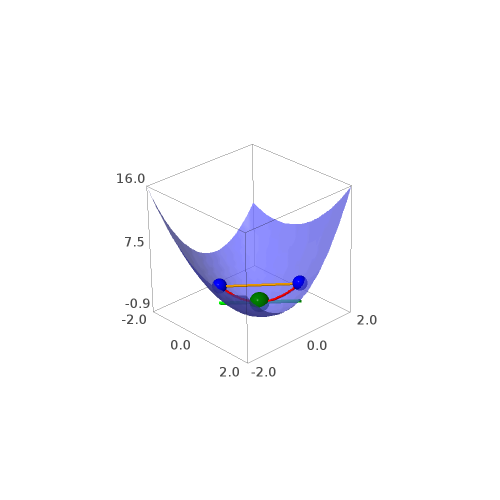
\includegraphics[width=0.25\textwidth]{imagens/lista04/picture_lista04.02_q03.png}
				\captionof{figure}{Exemplo do TVM, com função $f(x,y)=x^2 + xy + 2y^2$}
			\end{center}
		\end{solucao}
\end{document}
